\chapter{Data and Monte Carlo samples}\label{chap:DataSample}
\minitoc

\section{Collision data}

\begin{figure}[!b]
\begin{minipage}[h]{0.49\linewidth}
\center{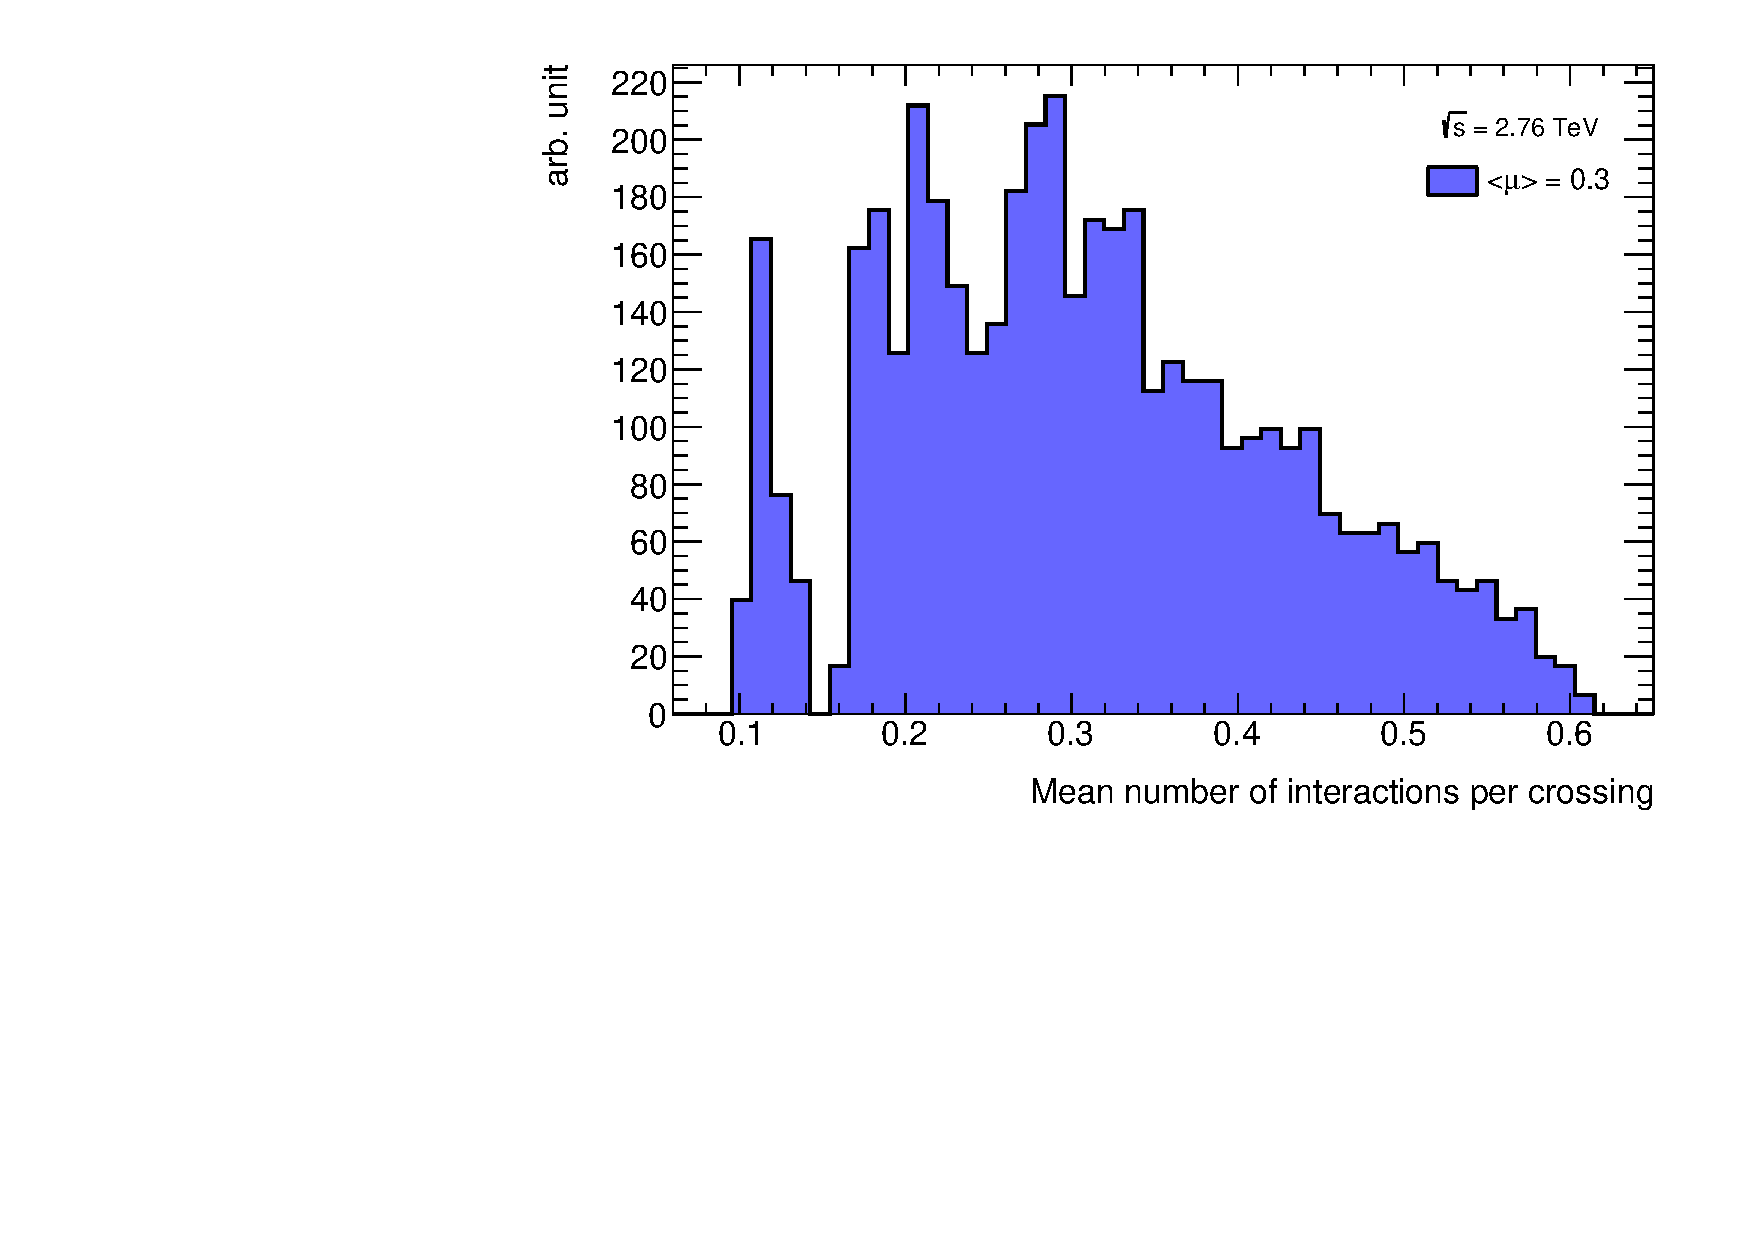
\includegraphics[width=1.\linewidth]{DataSample/mu.pdf}\\ a)}
\end{minipage}
\hfill
\begin{minipage}[h]{0.49\linewidth}
\center{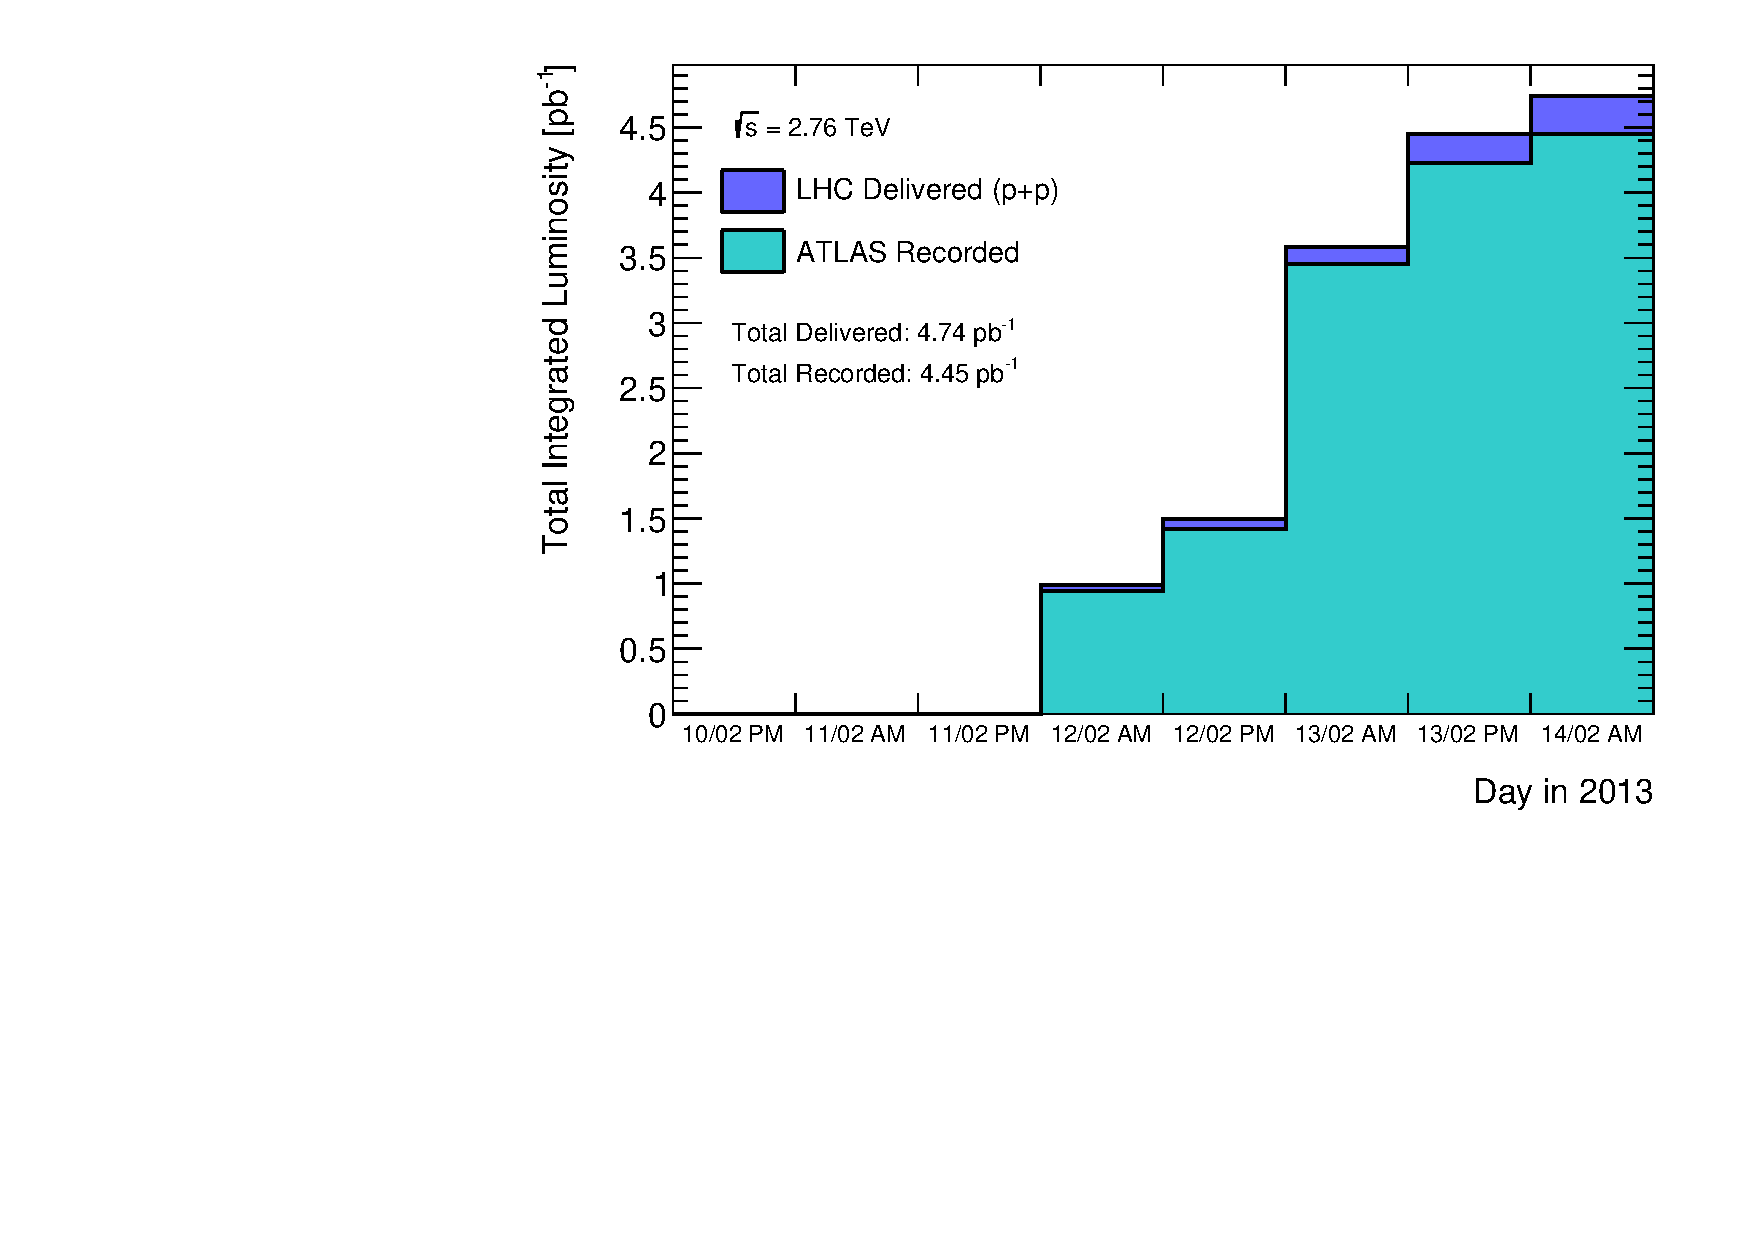
\includegraphics[width=1.\linewidth]{DataSample/lumi.pdf}\\ b)}
\end{minipage}
\caption{a) Mean number of interactions per bunch crossing and b) cumulative luminosity  delivered by LHC (dark blue) versus day, and recorded by ATLAS (light blue) for pp collisions at the center-of-mass energy 2.76 TeV in 2013.}
\label{ris:DataSampleMu}
\end{figure}
The data used in this analysis was collected in proton--proton (pp) collision runs at a center-of-mass energy 2.76 TeV at the LHC operation using the ATLAS detector. The mean number of interactions per bunch crossing for this runs is shown in Fig.~\ref{ris:DataSampleMu}. 

During these runs \atlas collected 4.45 pb$^{-1}$ of data (Fig.~\ref{ris:DataSampleMu} b). However, not all of the data is applicable for a precise physics analysis, so a set of additional data quality (DQ) requirements is applied.  Information about subdetectors that were disabled during data-taking is used. The information is stored in a Good Run List (GRL). The total luminosity of a data sample used in the analysis is 4.0 pb$^{-1}$ with the uncertainty  of 3.1\% \cite{myLumi}.

\section{Monte Carlo samples}

Simulated events are used to estimate both the signal and background processes contributions. A summary of the MC samples used in the analysis is given in Tab.~\ref{tab:MCSamples}. The primary signal samples are generated using Powheg generator with CT10\cite{NewPartonD} PDFs and showered with Pythia8 using AU2\cite{ATL-PHYS-PUB-2012-003} tune. Alternative signal MC samples are produced for W-analyses. They are generated using Sherpa with CT10 PDFs. This sample is used for studies of systematic errors coming from the choice of the generator (see Chap.~\ref{chap:Unc}).

The Monte Carlo samples are also used to estimate the fraction of background events in data. More detailed description of the background sources can be found in Chap.~\ref{chap:Backgr}. The $W\to \tau\nu$ and $Z \to \tau\tau$ processes are generated with Powheg+Pythia8 generator with CT10 PDF and AU2 tune. Events with diboson decays (WW, WZ, ZZ) are generated using Herwig with CTEQ6L1\cite{Pumplin2002} PDF set and AUET2\cite{ATL-PHYS-PUB-2010-014} tune. The top pair production ($t\bar{t}$) background is estimated using Powheg generator interfaced with Pythia6. The additional heavy quark pairs production ($b\bar{b}$ and $c\bar{c}$) samples needed for the multijet background determination (Sec.~\ref{sec:QCD}) are generated with Pythia8 with AU2 tune and CTEQ6L1 PDF set.

\begin{table}[!h]
\caption{Monte Carlo samples used to estimate signal and background processes.}
\label{tab:MCSamples}
\begin{center}
\begin{tabular}{l | c | c  }
Process & Generator & $N_{events}$ \\
\hline
\multicolumn{3}{c}{Signal MC}\\
\hline
$W^{+} \to e\nu$ & Powheg+Pythia8 & $2.0\cdot10^5$ \\
$W^{+} \to \mu\nu$ & Powheg+Pythia8 & $2.0\cdot10^5$ \\
$W^{-} \to e\nu$ & Powheg+Pythia8 & $1.2\cdot10^5$ \\
$W^{-} \to \mu\nu$ & Powheg+Pythia8 &  $1.2\cdot10^5$\\
$Z \to ee$ & Powheg+Pythia8 & $9.5\cdot10^4$ \\
$Z \to \mu\mu$ & Powheg+Pythia8 &  $7.0\cdot10^4$ \\
\hline
$W \to e\nu$ & Sherpa &  $4.9 \cdot 10^5$\\
$W \to \mu\nu$ & Sherpa &$4.8 \cdot 10^5$ \\
\hline 
\hline
\multicolumn{3}{c}{Background MC} \\
\hline
$W^{+} \to \tau\nu$ & Powheg+Pythia8 & $5.0\cdot10^4$ \\
$W^{-} \to \tau\nu$ & Powheg+Pythia8 & $3.0\cdot10^4$ \\
$Z \to \tau\tau$ & Powheg+Pythia8 & $2.0\cdot10^4$  \\
$t \bar{t}$ & Powheg+Pythia6 &  $5.0\cdot10^3$\\
$WW$ & Herwig &  $1.0\cdot10^3$ \\
$ZZ$ & Herwig &   $5.0\cdot10^3$ \\
$WZ$ & Herwig &  $1.0\cdot10^3$ \\
$b\bar{b}$ & Pythia8 & $5.0 \cdot 10^5$ \\
$c\bar{c}$ & Pythia8 &  $4.8 \cdot 10^5$ \\
\hline
\end{tabular}
\end{center}
\end{table}


